\documentclass{article}

% This is the preamble area where you include packages and set up document configurations
\usepackage[utf8]{inputenc} % For modern character encoding
\usepackage[T1]{fontenc} % T1 Font encoding
\usepackage{amsmath} % For mathematical symbols and environments
\usepackage{geometry} % For setting page dimensions and margins
\usepackage{graphicx} % For including images
\usepackage{hyperref} % For clickable links

% Set up page dimensions
\geometry{
 a4paper,
 total={170mm,257mm},
 left=20mm,
 top=20mm,
}

\title{My First Document}
\author{Your Name}
\date{\today} % This will print the current date

\begin{document}

\maketitle % This command creates the title using the information provided above

\section{Introduction}
This is the introduction to my first document created in \LaTeX.

\subsection{A Subsection}
Here's some more text under a subsection.

\paragraph{}
This is a new paragraph in your document. You can write your text here and when you want to start a new paragraph, just add another \textbackslash{}paragraph command.

If you want to include an image, use the following syntax:
\begin{figure}[ht]
\centering
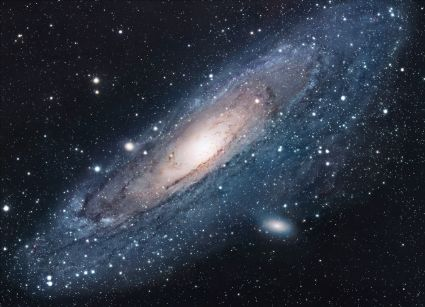
\includegraphics[width=0.8\textwidth]{universe.jpg}
\caption{A picture of the universe}
\label{fig:universe}
\end{figure}

\section{Conclusion}
This is the conclusion of my document.

\end{document}
